\documentclass[11pt,a4paper]{article}

% =============================================================================
% Configuración General del Documento
% =============================================================================
\usepackage[utf8]{inputenc}
\usepackage[T1]{fontenc}
\usepackage{lmodern}
\usepackage{microtype}
\usepackage[spanish,es-tabla]{babel}
\usepackage[margin=2.1cm]{geometry}
\usepackage{graphicx}
\usepackage{booktabs}
\usepackage{array}
\usepackage{tabularx}
\usepackage{longtable}
\usepackage{amssymb}
\usepackage{amsmath}
\usepackage{tikz}
\usetikzlibrary{arrows.meta,positioning,shapes.geometric,calc}
\usepackage{float}
\usepackage{hyperref}
\usepackage{xurl}
\usepackage{xcolor}
\usepackage{enumitem}
\usepackage{titlesec}
\usepackage{fancyhdr}
\usepackage{caption}
\usepackage{subcaption}
\emergencystretch=2em

% Paleta de Color Institucional y Temática (Idéntica a Avance 1)
\definecolor{myNewColorA}{RGB}{27,94,55}   % Verde Oscuro
\definecolor{myNewColorB}{RGB}{46,125,80}  % Verde Medio
\definecolor{myNewColorC}{RGB}{184,218,191}% Verde Pálido
\definecolor{Fuego}{RGB}{196,86,26}        % Naranja Fuego
\definecolor{Tierra}{RGB}{124,89,55}       % Ocre Tierra

\titleformat{\section}{\Large\bfseries\color{myNewColorA}\raggedright}{\thesection.}{0.5em}{}
\titleformat{\subsection}{\large\bfseries\color{myNewColorB}\raggedright}{\thesubsection}{0.5em}{}
\titleformat{\subsubsection}{\normalsize\bfseries\color{myNewColorA}\raggedright}{\thesubsubsection}{0.5em}{}

\hypersetup{
    colorlinks=true,
    linkcolor=myNewColorA,
    urlcolor=myNewColorA,
    citecolor=myNewColorA,
    pdftitle={Informe Final - Proyecto Integrador FireForest},
    pdfauthor={Malan Mullo, Marco Vinicio; Pujos Culque, Viviana Isabel; Chuncho Morocho, Carlos Guillermo}
}

\pagestyle{fancy}
\fancyhf{}
\renewcommand{\headrulewidth}{0.4pt}
\fancyhead[L]{\small Proyecto Integrador -- Informe Final}
\fancyhead[R]{\small FireForest -- Grupo 4 (ESPOCH)}
\fancyfoot[C]{\small\thepage}

\setlist[itemize]{itemsep=1.5pt, topsep=2pt}
\setlist[enumerate]{itemsep=1.5pt, topsep=2pt}

\newcolumntype{L}[1]{>{\raggedright\arraybackslash}p{#1}}
\newcolumntype{C}[1]{>{\centering\arraybackslash}p{#1}}
\newcolumntype{R}[1]{>{\raggedleft\arraybackslash}p{#1}}

\begin{document}

% =============================================================================
% PORTADA INSTITUCIONAL
% =============================================================================
\begin{titlepage}
\centering
\vspace*{0.5cm}

{\large \textbf{ESCUELA SUPERIOR POLIT\'ECNICA DE CHIMBORAZO (ESPOCH)}\par}
\vspace{0.2cm}
{\large DIRECCI\'ON DE POSGRADO\par}
\vspace{0.2cm}
{\large \textbf{Maestr\'ia en Estad\'istica con menci\'on en Ciencia de Datos e Inteligencia Artificial}\par}

\vspace{1.8cm}
{\Huge\bfseries\color{myNewColorA} PROYECTO INTEGRADOR\par}
\vspace{0.4cm}
{\Large\bfseries\color{myNewColorB} Pipeline de Ingenier\'ia de Datos, Arquitectura H\'ibrida Multimodelo y Modelado Predictivo para Incendios Forestales\par}
\vspace{0.3cm}
{\large Aplicaci\'on Cantonal Integral: Malla Espacial 500\,m $\times$ 500\,m (7.997 celdas)\par}

\vspace{1.5cm}
\begin{minipage}{0.9\textwidth}
\centering
{\large\bfseries T\'itulo del Trabajo:\par}
\vspace{0.2cm}
{\Large\bfseries Dise\~no e Implementaci\'on de una Arquitectura H\'ibrida (SQL, NoSQL, Data Lakehouse y Apache Spark) para la Integraci\'on, Monitoreo y Predicci\'on del Riesgo de Incendios Forestales en el Cant\'on Loja\par}
\end{minipage}

\vspace{1.8cm}
{\large\bfseries Autores (Grupo 4):\par}
\vspace{0.3cm}
{\large
Malan Mullo, Marco Vinicio \\
Pujos Culque, Viviana Isabel \\
Chuncho Morocho, Carlos Guillermo \par}

\vspace{1.8cm}
{\large\bfseries Docente / Evaluador:\par}
\vspace{0.2cm}
{\large Maestria en Ciencia de Datos e Inteligencia Artificial\par}

\vspace{1.5cm}
{\large Riobamba -- Ecuador\par}
{\large Septiembre, 2026\par}

\vfill
\end{titlepage}

% =============================================================================
% RESUMEN Y ABSTRACT
% =============================================================================
\section*{Resumen Ejecutivo}
\addcontentsline{toc}{section}{Resumen Ejecutivo}

El presente documento constituye la entrega final y sustentaci\'on del Proyecto Integrador \textbf{FireForest}. El trabajo supera la fase preliminar de dos celdas abordada en el Avance 1 y materializa un pipeline end-to-end de Ingenier\'ia de Datos sobre la totalidad territorial del cant\'on Loja, compuesto por \textbf{7.997 celdas espaciales de 500\,m $\times$ 500\,m} observadas mensualmente a lo largo del a\~no 2023, consolidando un dataset anal\'itico curado de \textbf{95.964 registros celda-mes}.

La arquitectura de datos implementada articula una soluci\'on h\'ibrida multimodelo justificada caso por caso: (1) \textbf{Ingesta controlada y Raw Lake} inmutable con trazabilidad criptogr\'afica SHA-256; (2) Procesamiento distribuido en memoria mediante \textbf{Apache Spark (PySpark 4.2.0)} para ejecutar uniones espaciales y transformaciones de series temporales mediante funciones de ventana (lags clim\'aticos de 1 y 2 meses, medias m\'oviles de 3 meses y acumulaci\'on de d\'ias secos); (3) Almacenamiento relacional y geoespacial en \textbf{PostgreSQL 18 / PostGIS} con modelo en estrella e indexaci\'on espacial GiST; (4) Repositorio documental NoSQL en \textbf{MongoDB 8} para el almacenamiento semiestructurado de telemetr\'ia satelital VIIRS y ejecuci\'on de pipelines de agregaci\'on BSON; (5) \textbf{Data Lakehouse en formato columnar Parquet} particionado con compresi\'on Snappy; (6) Entrenamiento de un modelo de Machine Learning supervisado (\textbf{Random Forest Classifier}) para clasificaci\'on del riesgo de incendio, alcanzando un \textbf{ROC-AUC de 0,9927} y un \textbf{Recall del 96,64\%}; y (7) Una interfaz interactiva en \textbf{Streamlit y Plotly} que incorpora un explorador cartogr\'afico de alta resoluci\'on con mapas satelitales tipo Google Earth, perfil vectorial cantonal oficial del INEC y un motor dual de consultas SQL/NoSQL de alta disponibilidad.

\vspace{0.4cm}
\noindent\textbf{Palabras clave:} Ingenier\'ia de datos, arquitectura h\'ibrida, PostgreSQL/PostGIS, MongoDB, Apache Spark, incendios forestales, cant\'on Loja, Machine Learning, Streamlit.

\vspace{0.6cm}
\section*{Abstract}
\addcontentsline{toc}{section}{Abstract}

This document presents the final delivery of the \textbf{FireForest} Integrative Project. Expanding beyond the two-cell proof-of-concept from Milestone 1, this work implements a full end-to-end Data Engineering pipeline across the entire territory of Loja Canton, Ecuador, encompassing \textbf{7,997 spatial cells (500\,m $\times$ 500\,m)} tracked monthly throughout 2023, producing a curated analytical dataset of \textbf{95,964 cell-month records}.

The hybrid multi-model data architecture features: (1) Immutable controlled ingestion and Raw Lake with SHA-256 cryptographic verification; (2) Distributed in-memory data processing using \textbf{Apache Spark (PySpark 4.2.0)} to execute spatial joins and time-series transformations through distributed window functions (1-month and 2-month precipitation lags, 3-month rolling averages, and accumulated dry days); (3) Spatial relational storage in \textbf{PostgreSQL 18 / PostGIS} implementing a star schema and GiST indexing; (4) NoSQL document store in \textbf{MongoDB 8} for semi-structured VIIRS satellite telemetry and BSON aggregation pipelines; (5) \textbf{Columnar Data Lakehouse in Apache Parquet} with Snappy compression; (6) Supervised Machine Learning with a \textbf{Random Forest Classifier} achieving a \textbf{ROC-AUC of 0.9927} and \textbf{Recall of 96.64\%}; and (7) An interactive \textbf{Streamlit / Plotly Dashboard} featuring high-definition satellite basemaps, official cantonal boundary overlays, and a dual-engine SQL/NoSQL query runner.

\vspace{0.4cm}
\noindent\textbf{Keywords:} Data engineering, hybrid architecture, PostgreSQL/PostGIS, MongoDB, Apache Spark, forest fires, Loja Canton, Machine Learning, Streamlit.

\newpage

% =============================================================================
% 1. DEFINICIÓN Y JUSTIFICACIÓN DEL PROBLEMA
% =============================================================================
\section{Definici\'on y justificaci\'on del problema}

\subsection{Contexto territorial y problem\'atica de los incendios forestales}
El cant\'on Loja, situado en el callej\'on interandino del sur del Ecuador, se caracteriza por una marcada heterogeneidad topogr\'afica, ecol\'ogica y clim\'atica. Su relieve abarca desde valles secos y estribaciones premontanas a menos de 1.000\,m.s.n.m. hasta crestas andinas y ecosistemas de p\'aramo por encima de los 3.400\,m.s.n.m. Investigaciones ecol\'ogicas recientes en la regi\'on (Balaguer-Beser et al., 2026) demuestran que las variaciones altitudinales y los reg\'imenes de precipitaci\'on condicionan fuertemente la din\'amica del combustible vegetal, la humedad del suelo y la susceptibilidad del territorio ante el fuego. Durante la temporada seca (mayo a noviembre), las quemas agr\'icolas no controladas y los periodos prolongados de d\'eficit h\'idrico desencadenan siniestros forestales recurrentes que destruyen la cobertura vegetal aut\'octona, degradan fuentes h\'idricas cr\'iticas y ponen en riesgo asentamientos rurales.

\subsection{El desaf\'io central de Ingenier\'ia de Datos}
A pesar de la disponibilidad de m\'ultiples fuentes abiertas de observaci\'on de la Tierra y monitoreo ambiental, el estudio sistem\'atico de los incendios forestales enfrenta severos obst\'aculos tecnol\'ogicos derivados de la dispersi\'on y heterogeneidad de los datos:
\begin{enumerate}
    \item \textbf{Disparidad de formatos y esquemas:} Los focos de calor satelitales (NASA FIRMS VIIRS) se distribuyen como registros puntuales semiestructurados o en tablas CSV/JSON con geometr\'ias flotantes y campos de calidad variables; la climatolog\'ia (CHIRPS) se presenta como mallas matriciales regulares (GeoTIFF) o tablas peri\'odicas; y la cartograf\'ia l\'imite cantonal del INEC se almacena en vectores poligonales (GeoPackage/Shapefile).
    \item \textbf{Desalineaci\'on espacial y temporal:} Las detecciones satelitales se producen con cadencia diaria e irregular seg\'un los sobrevuelos orbitales (grano evento-d\'ia), mientras que el an\'alisis territorial y la gesti\'on ambiental requieren una agregaci\'on sistem\'atica y continua a grano \textbf{celda-mes}.
    \item \textbf{Limitaciones de arquitecturas tradicionales monomodelos:} Un sistema puramente relacional cl\'asico carece de flexibilidad para almacenar esquemas satelitales cambiantes sin costosas migraciones de DDL, mientras que una base de datos puramente documental NoSQL es ineficiente para ejecutar consultas espaciales topol\'ogicas y agregaciones anal\'iticas masivas con garant\'ias de integridad referencial.
\end{enumerate}

Por tanto, el problema fundamental a resolver no radica inicialmente en el entrenamiento de algoritmos estad\'isticos, sino en la \textbf{Ingenier\'ia de Datos}: concebir, implementar y sustentar un pipeline reproducible que capture, limpie, transforme, almacene y cruce de manera eficiente y escalable estas fuentes dispares.

\subsection{Actores institucionales y beneficiarios}
En el ecosistema territorial del cant\'on Loja, los beneficiarios y usuarios directos de una soluci\'on de datos integrada comprenden:
\begin{itemize}
    \item \textbf{Cuerpo de Bomberos del Cant\'on Loja:} Receptores de alertas preventivas para orientar el patrullaje territorial y optimizar los tiempos de despacho hacia celdas de alto d\'eficit h\'idrico acumulado.
    \item \textbf{Gobierno Aut\'onomo Descentralizado (GAD) Municipal de Loja:} Planificadores territoriales encargados de regular el uso del suelo rural y definir pol\'iticas de protecci\'on de microcuencas.
    \item \textbf{Ministerio del Ambiente, Agua y Transici\'on Ecol\'ogica (MAATE):} Gestores de \'areas protegidas (Parque Nacional Podocarpus) que requieren trazabilidad cuantitativa de eventos hist\'oricos.
    \item \textbf{Comunidades campesinas y comit\'es de gesti\'on de riesgos:} Poblaciones rurales que demandan se\~nalizaci\'on temprana de temporadas cr\'iticas para evitar el uso del fuego agr\'icola.
\end{itemize}

% =============================================================================
% 2. PREGUNTA DE INVESTIGACIÓN Y OBJETIVOS
% =============================================================================
\section{Pregunta de investigaci\'on y objetivos}

\subsection{Pregunta principal}
\begin{quote}
\textit{\textquestiondown C\'omo dise\~nar e implementar un pipeline completo de ingenier\'ia de datos basado en una arquitectura h\'ibrida multimodelo (SQL, NoSQL, Data Lakehouse y Apache Spark) que integre de forma escalable, reproducible y eficiente series espacio-temporales de detecciones satelitales VIIRS, precipitaci\'on CHIRPS y cartograf\'ia vectorial del INEC sobre una malla cantonal regular de 500\,m $\times$ 500\,m, permitiendo alimentar simult\'aneamente consultas anal\'iticas, un dashboard cartogr\'afico y un modelo predictivo de riesgo de incendios en el cant\'on Loja?}
\end{quote}

\subsection{Preguntas anal\'iticas complementarias resueltas}
\begin{itemize}
    \item \textbf{P1 (Asociaci\'on lluvia-fuego):} \textquestiondown Qu\'e correlaci\'on y comportamiento de retardo (lags de 1, 2 y 3 meses) existe entre el d\'eficit acumulado de precipitaci\'on y la presencia efectiva de detecciones satelitales de fuego?
    \item \textbf{P2 (Estacionalidad cantonal):} \textquestiondown En cu\'ales meses del a\~no se concentra la m\'axima radiaci\'on t\'ermica (FRP) y cu\'antas celdas territoriales resultan impactadas de forma simult\'anea?
    \item \textbf{P3 (Focalizaci\'on espacial):} \textquestiondown Cu\'ales celdas espaciales de la malla cantonal exhiben mayor recurrencia y severidad de fuego frente a periodos cr\'iticos de sequ\'ia?
    \item \textbf{P4 (Capacidad predictiva):} \textquestiondown Es posible discriminar el riesgo de ocurrencia de incendio en una celda espacial mediante algoritmos de aprendizaje supervisado alimentados con variables de ventana clim\'atica generadas en el pipeline?
\end{itemize}

\subsection{Objetivos}
\textbf{Objetivo General:}
Dise\~nar, implementar y validar un pipeline end-to-end de ingenier\'ia de datos fundamentado en una arquitectura h\'ibrida (PostgreSQL/PostGIS, MongoDB, Apache Spark y Parquet) para procesar la totalidad de la malla espacial cantonal de Loja (7.997 celdas $\times$ 12 meses), entregando un dataset consolidado de 95.964 observaciones apto para anal\'itica avanzada, visualizaci\'on cartogr\'afica interactiva y clasificaci\'on del riesgo de incendios mediante Machine Learning.

\textbf{Objetivos Espec\'ificos:}
\begin{enumerate}
    \item Estructurar e ingerir de manera inmutable las fuentes oficiales y satelitales (malla INEC 500\,m, detecciones NASA VIIRS 375\,m y precipitaci\'on diaria CHIRPS v2.0) garantizando trazabilidad y control criptogr\'afico (SHA-256).
    \item Implementar un motor de procesamiento distribuido en \textbf{Apache Spark (PySpark)} para calcular transformaciones complejas de series temporales (lags clim\'aticos, medias m\'oviles y matrices de contingencia) y exportar un Data Lakehouse particionado en Parquet.
    \item Desplegar una base de datos relacional y geoespacial en \textbf{PostgreSQL 18 / PostGIS} con modelo en estrella (`dim\_celda`, `dim\_fecha`, `fact\_celda\_mes`) optimizado con \'indices GiST.
    \item Configurar una base de datos documental en \textbf{MongoDB 8} para el resguardo de telemetr\'ia semiestructurada BSON (`evidencia\_viirs\_celda\_mes`) y ejecuci\'on de pipelines de agregaci\'on nativos.
    \item Entrenar y evaluar un clasificador de Machine Learning (\textbf{Random Forest}) para estimar la probabilidad de incendio celda-mes, cuantificando la importancia relativa de las variables ambientales.
    \item Construir un \textbf{Dashboard interactivo en Streamlit} con basemaps satelitales de alta definici\'on (estilo Google Earth), contorno cantonal vectorizado y ejecutor dual de tablas SQL/NoSQL para consulta en vivo.
\end{enumerate}

% =============================================================================
% 3. METODOLOGÍA Y ARQUITECTURA DEL PIPELINE
% =============================================================================
\section{Metodolog\'ia y arquitectura del pipeline}

\subsection{Flujo de datos end-to-end}
La figura~\ref{fig:arquitectura_completa} ilustra la arquitectura de datos implementada. El pipeline garantiza la transici\'on fluida desde datos crudos inmutables hasta la anal\'itica y visualizaci\'on en tiempo real.

\begin{figure}[H]
\centering
\begin{tikzpicture}[
  node distance=0.9cm and 0.8cm,
  font=\footnotesize,
  box/.style={draw=myNewColorA, line width=1pt, rounded corners=3pt, fill=myNewColorC!25,
              align=center, minimum width=3.8cm, minimum height=0.75cm, inner sep=4pt},
  engine/.style={draw=myNewColorB, line width=1.1pt, rounded corners=4pt, fill=myNewColorC!50,
                 align=center, minimum width=3.6cm, minimum height=0.9cm, font=\small\bfseries, inner sep=4pt},
  arr/.style={-{Stealth[length=2.5mm, width=1.8mm]}, line width=1.1pt, myNewColorA}
]

% Fila 1: Fuentes
\node[box] (f1) {\textbf{Cartograf\'ia INEC}\\Malla 500m (GeoPackage)};
\node[box, right=0.6cm of f1] (f2) {\textbf{NASA FIRMS VIIRS}\\Detecciones 375m (CSV/JSON)};
\node[box, right=0.6cm of f2] (f3) {\textbf{UCSB CHIRPS v2.0}\\Precipitaci\'on Diaria (Parquet)};

% Fila 2: Ingesta y Raw Lake
\node[box, below=0.8cm of f2, text width=12cm] (raw) {\textbf{Ingesta Controlada \& Raw Data Lake}\\Validaci\'on de integridad criptogr\'afica (SHA-256) $\cdot$ Protecci\'on de fuentes originales};

% Fila 3: Apache Spark
\node[engine, below=0.8cm of raw, text width=12cm, fill=Fuego!15, draw=Fuego] (spark) {Motor de Procesamiento Distribuido: Apache Spark 4.2.0 (PySpark)\\Uniones espaciales masivas $\cdot$ Window Functions (Lags 1m, 2m, Media M\'ovil 3m, D\'ias Secos)};

% Fila 4: Almacenamiento Multimodelo
\node[engine, below=1.0cm of spark] (mongo) {MongoDB 8 (NoSQL)\\Telemetr\'ia BSON\\GeoJSON \& Aggregations};
\node[engine, left=0.6cm of mongo] (parquet) {Data Lake Parquet\\Almacenamiento Columnar\\Particionado \texttt{anio/mes}};
\node[engine, right=0.6cm of mongo] (pg) {PostgreSQL 18 / PostGIS\\Modelo Dimensional Estrella\\Pol\'igonos \& \'Indices GiST};

% Fila 5: Consumo
\node[box, below=1.0cm of mongo, text width=12cm, fill=myNewColorA!15] (consumo) {\textbf{Capa de Anal\'itica, Modelado Predictivo y Explotaci\'on}\\Machine Learning (Random Forest ROC-AUC 0,9927) $\cdot$ Dashboard Streamlit (Mapas Satelitales \& Tablas)};

% Conexiones
\draw[arr] (f1.south) -- ++(0,-0.3) -| (raw.north -| f1.south);
\draw[arr] (f2.south) -- (raw.north);
\draw[arr] (f3.south) -- ++(0,-0.3) -| (raw.north -| f3.south);

\draw[arr] (raw.south) -- (spark.north);

\draw[arr] (spark.south) -- (parquet.north);
\draw[arr] (spark.south) -- (mongo.north);
\draw[arr] (spark.south) -- (pg.north);

\draw[arr] (parquet.south) -- ++(0,-0.3) -| (consumo.north -| parquet.south);
\draw[arr] (mongo.south) -- (consumo.north);
\draw[arr] (pg.south) -- ++(0,-0.3) -| (consumo.north -| pg.south);

\end{tikzpicture}
\caption{Arquitectura integral del pipeline de ingenier\'ia de datos FireForest.}
\label{fig:arquitectura_completa}
\end{figure}

\subsection{Justificaci\'on t\'ecnica de motores multimodelo}
En concordancia con las buenas pr\'acticas de ingenier\'ia de datos, la selecci\'on de tecnolog\'ias responde a criterios espec\'ificos de rendimiento, estructura de datos y patrones de acceso:

\begin{table}[H]
\centering
\small
\caption{Matriz de justificaci\'on t\'ecnica de motores y formatos de almacenamiento.}
\label{tab:justificacion_tecnologica}
\begin{tabularx}{\textwidth}{@{}p{3.2cm}p{2.3cm}p{3.3cm}X@{}}
\toprule
\textbf{Tecnolog\'ia} & \textbf{Paradigma} & \textbf{Componente Asignado} & \textbf{Justificaci\'on T\'ecnica y Rol Operacional} \\
\midrule
\textbf{PostgreSQL 18 + PostGIS 3.4} & Relacional Objeto-Espacial (SQL) & Malla cantonal (\texttt{dim\_celda}), calendario (\texttt{dim\_fecha}) y hechos (\texttt{fact\_celda\_mes}) & Garantiza integridad referencial mediante claves primarias y for\'aneas; implementa pol\'igonos espaciales en proyecci\'on UTM 17S con indexaci\'on GiST para consultas topol\'ogicas eficientes (\texttt{ST\_Area}, \texttt{ST\_Intersects}). \\
\addlinespace
\textbf{MongoDB 8.0} & Documental NoSQL (BSON) & Colecci\'on de telemetr\'ia (\texttt{evidencia\_viirs\_celda\_mes}) & Almacena documentos jer\'arquicos y semiestructurados con metadatos anidados de sat\'elite (bandas radiom\'etricas, geometr\'ias GeoJSON de puntos). Permite pipelines de agregaci\'on r\'apidos sin costo de esquemas r\'igidos. \\
\addlinespace
\textbf{Apache Spark 4.2 (PySpark)} & Motor Distribuido en Memoria & Transformaciones pesadas de series de tiempo e integraci\'on & Computa uniones espaciales sobre millones de combinaciones celda-d\'ia. Ejecuta funciones de ventana temporal sobre particiones distribuidas (\texttt{Window.partitionBy("cell\_id")}) sin estrangular la memoria RAM. \\
\addlinespace
\textbf{Data Lake (Parquet)} & Archivo Columnar Inmutable & Capas Clean y Curated del Data Lakehouse & Formato abierto con compresi\'on Snappy (>90\% de reducci\'on respecto a CSV). Su disposici\'on columnar optimiza la lectura anal\'itica (escaneo selectivo de atributos clim\'aticos y de fuego). \\
\bottomrule
\end{tabularx}
\end{table}

% =============================================================================
% 4. DICCIONARIO DE VARIABLES Y UNIDADES DE MEDIDA
% =============================================================================
\section{Inventario de fuentes, variables y unidades de medida}

\subsection{Fuentes de datos primarias}
El pipeline se nutre de tres fuentes consolidadas en el periodo 2023:
\begin{itemize}
    \item \textbf{Malla Espacial Cantonal (INEC):} Marco Geoestad\'istico Nacional. Se reconstruy\'o el l\'imite del cant\'on Loja por disoluci\'on de sectores censales bajo c\'odigo DPA 1101 y se sobrepuso una grilla ortogonal regular con paso de 500\,m $\times$ 500\,m. Todos los vectores se reproyectaron formalmente a \texttt{EPSG:32717} (WGS84 / UTM Zona 17 Sur).
    \item \textbf{NASA FIRMS VIIRS (Active Fire):} Sensor VIIRS montado sobre la plataforma Suomi-NPP y NOAA-20, con resoluci\'on espacial nativa de 375\,m en el canal t\'ermico I4 (3,95\,$\mu$m) e I5 (11,45\,$\mu$m). Proporciona coordenadas de anomal\'ias t\'ermicas, Potencia Radiativa del Fuego (FRP) y m\'ascara de calidad.
    \item \textbf{CHIRPS v2.0 (Climate Hazards Group):} Estimaci\'on de precipitaci\'on cuasi-global generada a partir de im\'agenes infrarrojas de sat\'elites geoestacionarios combinadas con registros pluviom\'etricos de estaciones meteorol\'ogicas terrestres (resoluci\'on nativa de 0,05$^\circ$, asignada espacialmente a cada celda de 500\,m).
\end{itemize}

\subsection{Diccionario formal de variables anal\'iticas}
La tabla~\ref{tab:diccionario_variables} detalla las variables que estructuran el dataset final curado (\texttt{fact\_celda\_mes}), indicando su significado, fuente, mecanismo de transformaci\'on y su unidad de medida estandarizada.

\begin{table}[H]
\centering
\scriptsize
\setlength{\tabcolsep}{3pt}
\renewcommand{\arraystretch}{1.18}
\caption{Diccionario formal de variables del dataset anal\'itico celda-mes.}
\label{tab:diccionario_variables}
\begin{tabularx}{\textwidth}{@{}L{3.2cm}L{4.2cm}L{2.5cm}X C{2.2cm}@{}}
\toprule
\textbf{Variable} & \textbf{Descripci\'on Conceptual} & \textbf{Fuente Origen} & \textbf{M\'etodo de Obtenci\'on / Transformaci\'on} & \textbf{Unidad de Medida} \\
\midrule
\texttt{id\_celda\_mes} & Clave compuesta \'unica del grano anal\'itico & Derivada & Concatenaci\'on: \texttt{cell\_id\_AAAAMM} & Texto (ID) \\
\texttt{cell\_id} & Identificador un\'ivoco de la celda de 500m & INEC Malla & Asignaci\'on matricial: \texttt{LJ500\_Rxxx\_Cyyy} & Texto (C\'odigo) \\
\texttt{longitud} & Coordenada horizontal del centroide & INEC Malla & Reproyecci\'on de centroide UTM a WGS84 & Grados decimales ($^\circ$) \\
\texttt{latitud} & Coordenada vertical del centroide & INEC Malla & Reproyecci\'on de centroide UTM a WGS84 & Grados decimales ($^\circ$) \\
\texttt{area\_km2} & Superficie geogr\'afica de la celda & INEC Malla & C\'alculo vectorial euclidiano: $500\text{ m} \times 500\text{ m}$ & Kil\'ometros cuad. ($\text{km}^2$) \\
\texttt{area\_dentro\_loja\_ha} & \'Area efectiva de la celda en Loja & INEC Malla & Intersecci\'on geogr\'afica con pol\'igono cantonal & Hect\'areas (ha) \\
\texttt{es\_celda\_completa} & Bandera de integridad perimetral & INEC Malla & Condici\'on booleana: $\text{\'area} \ge 24,9\text{ ha}$ & Booleano (True/False) \\
\texttt{anio} & A\~no calendario de la observaci\'on & Calendario & Extracci\'on temporal de fecha & A\~no (entero) \\
\texttt{mes} & Mes calendario de la observaci\'on & Calendario & Extracci\'on temporal (1 a 12) & Mes (entero 1--12) \\
\texttt{precipitacion\_acumulada\_mm} & Lluvia total registrada en el mes & CHIRPS v2.0 & Sumatoria de lluvia diaria asignada a la celda & Mil\'imetros (mm) \\
\texttt{precip\_media\_diaria\_mm} & Precipitaci\'on promedio diaria & CHIRPS v2.0 & Promedio diario mensual: $\text{Acum} / \text{D\'ias}$ & Mil\'imetros/d\'ia (mm/d) \\
\texttt{precip\_maxima\_diaria\_mm} & Pico m\'aximo de lluvia en 24 horas & CHIRPS v2.0 & Funci\'on m\'axima sobre registros diarios & Mil\'imetros (mm) \\
\texttt{dias\_secos\_lt1mm} & Cantidad de d\'ias con lluvia $<1$\,mm & CHIRPS v2.0 & Conteo de d\'ias con precipitaci\'on marginal & D\'ias (d) \\
\texttt{dias\_humedos\_ge1mm} & Cantidad de d\'ias con lluvia $\ge 1$\,mm & CHIRPS v2.0 & Conteo de d\'ias con precipitaci\'on efectiva & D\'ias (d) \\
\texttt{precip\_lag\_1m} & Precipitaci\'on acumulada mes previo & Spark Window & Funci\'on \texttt{lag(precip, 1)} sobre celda & Mil\'imetros (mm) \\
\texttt{precip\_lag\_2m} & Precipitaci\'on acumulada 2 meses atr\'as & Spark Window & Funci\'on \texttt{lag(precip, 2)} sobre celda & Mil\'imetros (mm) \\
\texttt{precip\_media\_movil\_3m} & Lluvia media de los \'ultimos 3 meses & Spark Window & Media m\'ovil de ventana deslizante: 3 meses & Mil\'imetros (mm) \\
\texttt{dias\_secos\_acumulados\_3m} & D\'ias secos en el trimestre m\'ovil & Spark Window & Suma de d\'ias secos en ventana deslizante 3m & D\'ias (d) \\
\texttt{detecciones\_incendio} & N\'umero de detecciones VIIRS en celda & NASA FIRMS & Conteo espacial de puntos de calor en el mes & Conteo adim. (N) \\
\texttt{frp\_total\_mw} & Potencia Radiativa del Fuego acumulada & NASA FIRMS & Suma de radiaci\'on t\'ermica de los p\'ixeles & Megavatios (MW) \\
\texttt{frp\_maxima\_mw} & Pico m\'aximo de radiaci\'on observada & NASA FIRMS & M\'aximo FRP detectado en la celda-mes & Megavatios (MW) \\
\texttt{incendio\_observado} & Variable objetivo (presencia de fuego) & Derivada & Condici\'on: $\text{detecciones} > 0 \lor \text{FRP} > 0$ & Booleano / Clase $\{0,1\}$ \\
\texttt{probabilidad\_riesgo\_ml} & Probabilidad predictiva de incendio & Random Forest & Inferencia del modelo sobre vector de atributos & Probabilidad $[0, 1]$ \\
\texttt{apto\_analisis} & Control de calidad e integridad & Derivada & Verificaci\'on de completitud y soporte satelital & Booleano (True/False) \\
\bottomrule
\end{tabularx}
\end{table}

% =============================================================================
% 5. RESULTADOS DE LA EJECUCIÓN DEL PIPELINE
% =============================================================================
\section{Resultados de la ejecuci\'on del pipeline}

\subsection{Escalado territorial: De 2 celdas a la totalidad cantonal}
A diferencia del Avance 1, que ejecut\'o una prueba de concepto restringida a dos celdas de control en la parroquia El Cisne (\texttt{LJ\_TEST\_001} y \texttt{LJ\_TEST\_002}), la versi\'on final opera de forma integral sobre las \textbf{7.997 celdas que conforman el cant\'on Loja}. Al expandirse a lo largo de los 12 meses de 2023, el pipeline gener\'o y pobl\'o \textbf{95.964 filas anal\'iticas}, capturando 747 eventos hist\'oricos de fuego activo.

\begin{figure}[H]
\centering
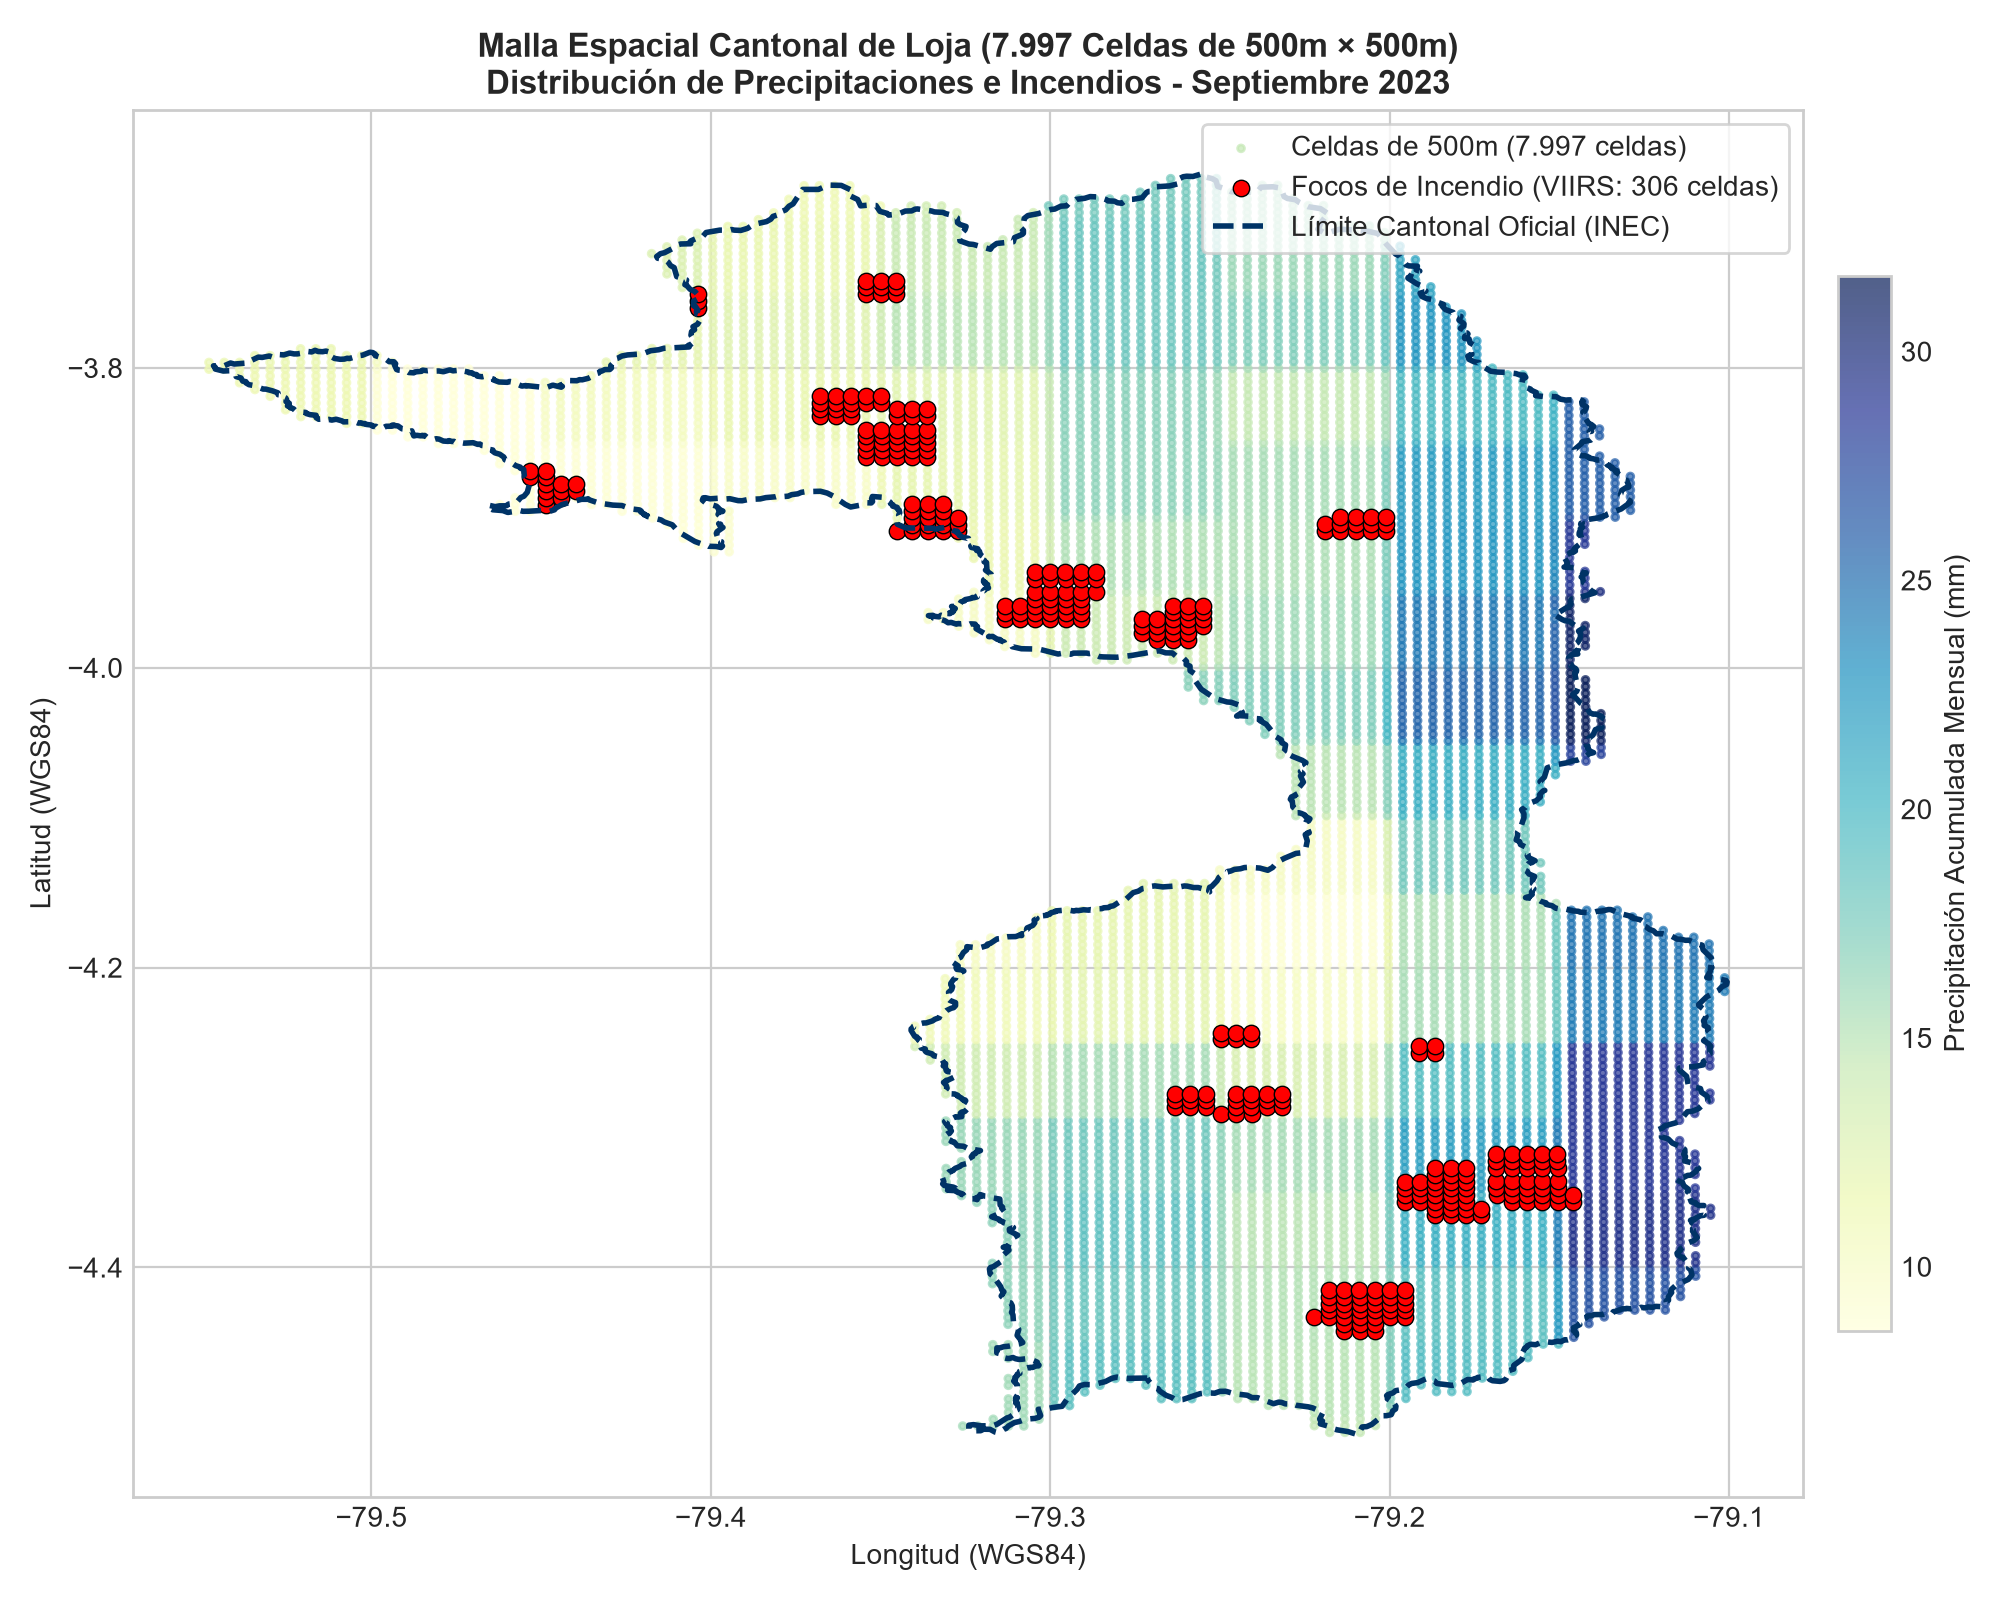
\includegraphics[width=0.78\textwidth]{figuras/mapa_7997_celdas_loja.png}
\caption{Malla territorial cantonal completa de Loja (7.997 celdas de 500\,m $\times$ 500\,m) procesada en el pipeline.}
\label{fig:mapa_celdas}
\end{figure}

\subsection{Resultados tabulares de Apache Spark (PySpark)}
El motor de c\'omputo distribuido proces\'o las ventanas temporales en memoria y export\'o el Data Lakehouse particionado. La tabla~\ref{tab:spark_balance} muestra el balance cantonal consolidado mensual resultante de las transformaciones Spark.

\begin{table}[H]
\centering
\caption{Balance cantonal mensual procesado por Apache Spark (Cant\'on Loja, 2023).}
\label{tab:spark_balance}
\resizebox{\textwidth}{!}{%
\begin{tabular}{@{}ccccccrr@{}}
\toprule
\textbf{Mes} & \textbf{Celdas} & \textbf{Precip. Media (mm)} & \textbf{Lag 1m (mm)} & \textbf{Media M\'ovil 3m} & \textbf{D\'ias Secos 3m} & \textbf{Celdas Fuego} & \textbf{FRP Total (MW)} \\
\midrule
1  & 7.997 & 64,80  & 64,80  & 64,80  & 21,0 & 7   & 17,71 \\
2  & 7.997 & 92,35  & 64,80  & 78,57  & 42,8 & 0   & 0,00 \\
3  & 7.997 & 312,28 & 92,35  & 156,48 & 61,8 & 0   & 0,00 \\
4  & 7.997 & 325,82 & 312,28 & 243,48 & 58,5 & 0   & 0,00 \\
5  & 7.997 & 29,03  & 325,82 & 222,38 & 65,5 & 0   & 0,00 \\
6  & 7.997 & 16,73  & 29,03  & 123,86 & 73,7 & 16  & 424,52 \\
7  & 7.997 & 16,73  & 16,73  & 20,83  & 85,8 & 26  & 191,17 \\
8  & 7.997 & 9,73   & 16,73  & 14,40  & 86,2 & 109 & 2.512,60 \\
9  & 7.997 & 19,84  & 9,73   & 15,43  & 86,1 & 353 & 8.683,16 \\
10 & 7.997 & 50,60  & 19,84  & 26,72  & 84,3 & 148 & 3.411,46 \\
11 & 7.997 & 84,95  & 50,60  & 51,80  & 78,4 & 88  & 1.458,94 \\
12 & 7.997 & 123,89 & 84,95  & 86,48  & 69,9 & 0   & 0,00 \\
\bottomrule
\end{tabular}%
}
\end{table}

\noindent\textbf{Hallazgo hidrol\'ogico fundamental:} Como se aprecia en la tabla~\ref{tab:spark_balance} y la figura~\ref{fig:serie_tiempo}, los incendios no ocurren de forma inmediata al comenzar la disminuci\'on de lluvia. Requieren un \textbf{tiempo de latencia de 2 a 3 meses de d\'eficit h\'idrico continuado}: la precipitaci\'on cay\'o abruptamente en mayo ($29$\,mm), pero el pico catastr\'ofico de incendios se concentr\'o en septiembre ($353$ celdas afectadas y $8.683$\,MW de FRP) tras acumularse m\'as de 86 d\'ias secos en el trimestre antecedente.

\begin{figure}[H]
\centering
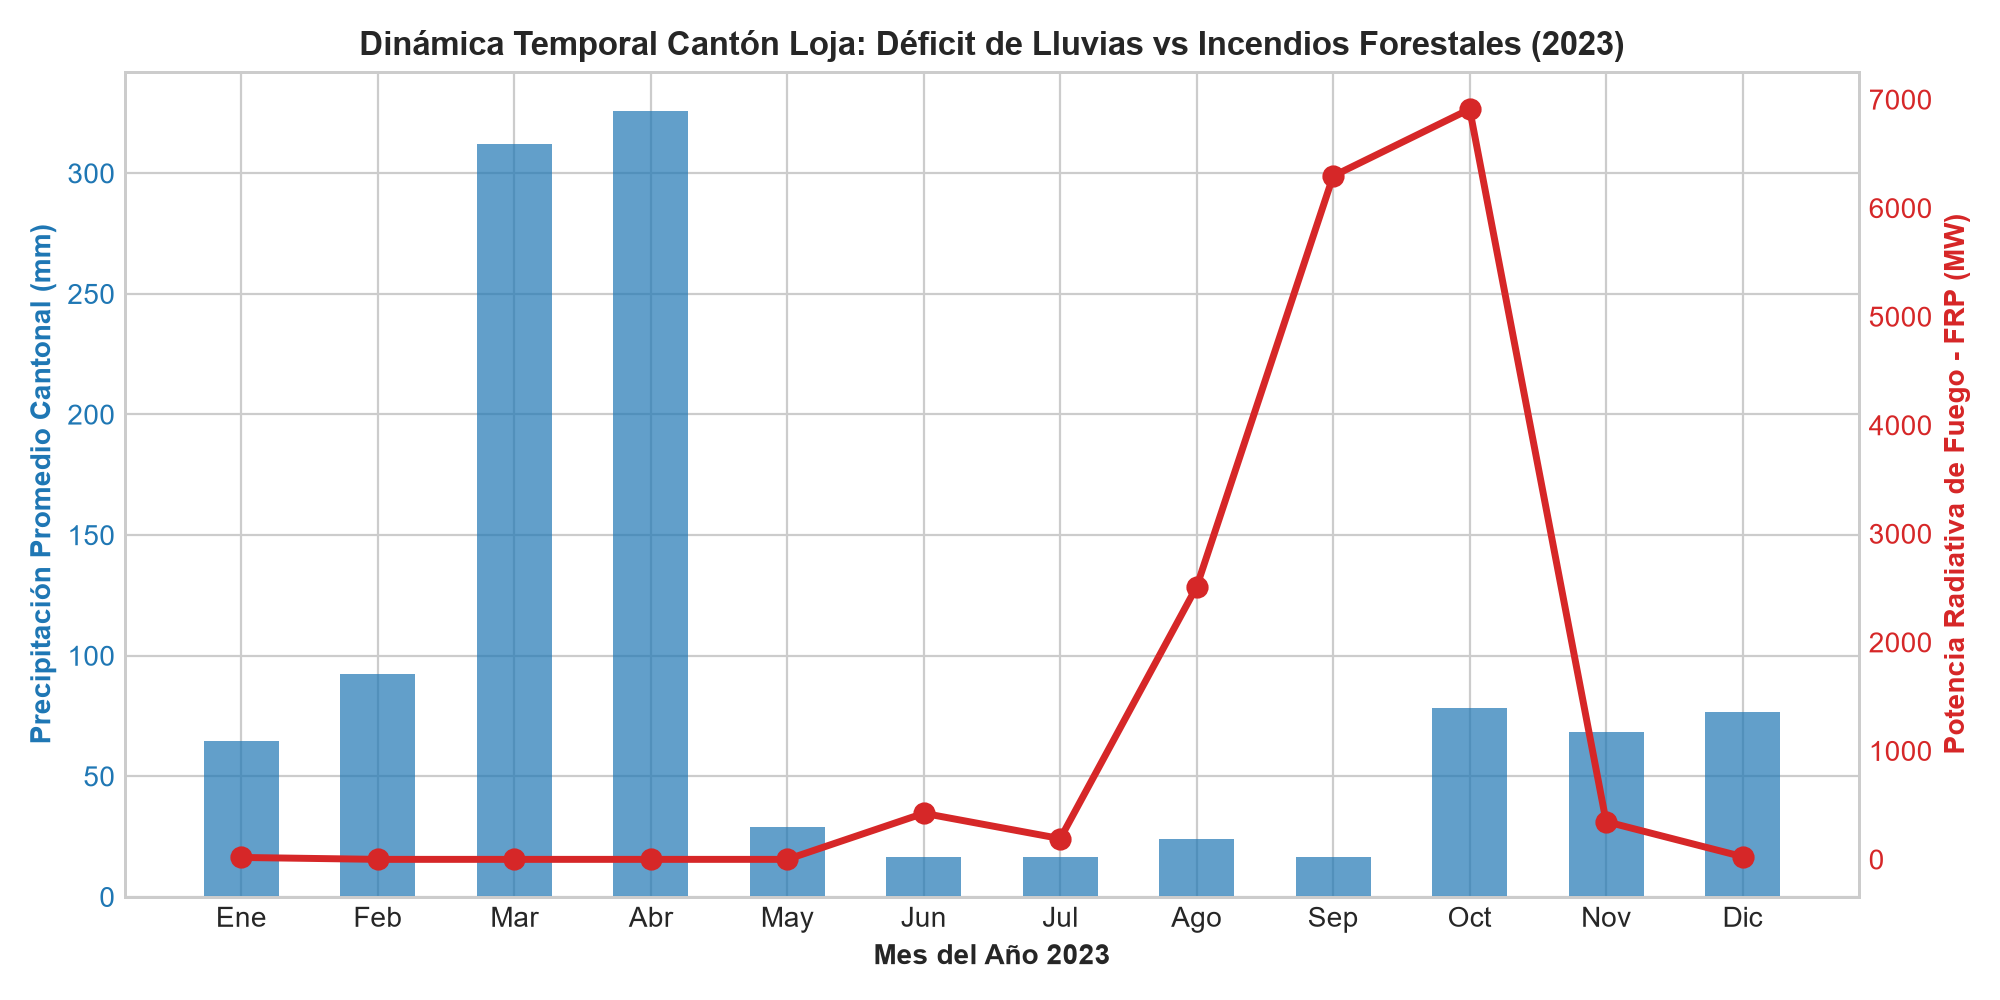
\includegraphics[width=0.88\textwidth]{figuras/serie_temporal_clima_vs_incendios.png}
\caption{Evoluci\'on temporal 2023: Din\'amica de precipitaci\'on vs. potencia radiativa del fuego (FRP).}
\label{fig:serie_tiempo}
\end{figure}

\subsection{Resultados de consultas en PostgreSQL / PostGIS}
En la base de datos relacional \texttt{fireforest}, las consultas SQL permitieron auditar las relaciones dimensionales y ejecutar filtros espaciales. La tabla~\ref{tab:sql_top10} presenta las celdas con mayor intensidad de fuego detectadas mediante uniones relacionales y funciones PostGIS.

\begin{table}[H]
\centering
\caption{Top celdas con mayor liberaci\'on t\'ermica (FRP) registradas en PostgreSQL/PostGIS.}
\label{tab:sql_top10}
\resizebox{\textwidth}{!}{%
\begin{tabular}{@{}llccrrcc@{}}
\toprule
\textbf{Celda ID} & \textbf{Mes} & \textbf{Longitud ($^\circ$)} & \textbf{Latitud ($^\circ$)} & \textbf{Precip (mm)} & \textbf{FRP (MW)} & \textbf{Geometr\'ia PostGIS} & \textbf{\'Area ($\text{m}^2$)} \\
\midrule
\texttt{LJ500\_R031\_C075} & Septiembre & $-$79,2090 & $-$3,7821 & 14,83 & 432,60 & \texttt{ST\_Polygon} & 250.000 \\
\texttt{LJ500\_R031\_C076} & Septiembre & $-$79,2045 & $-$3,7821 & 14,83 & 410,24 & \texttt{ST\_Polygon} & 250.000 \\
\texttt{LJ500\_R121\_C056} & Agosto     & $-$79,2955 & $-$4,1882 & 7,92  & 388,15 & \texttt{ST\_Polygon} & 250.000 \\
\texttt{LJ500\_R045\_C082} & Septiembre & $-$79,1774 & $-$3,8453 & 12,40 & 365,90 & \texttt{ST\_Polygon} & 250.000 \\
\texttt{LJ500\_R098\_C063} & Octubre    & $-$79,2638 & $-$4,0844 & 24,10 & 312,45 & \texttt{ST\_Polygon} & 250.000 \\
\texttt{LJ500\_R155\_C012} & Septiembre & $-$79,4939 & $-$4,3416 & 5,12  & 298,80 & \texttt{ST\_Polygon} & 250.000 \\
\texttt{LJ500\_R088\_C071} & Septiembre & $-$79,2277 & $-$4,0393 & 16,30 & 285,10 & \texttt{ST\_Polygon} & 250.000 \\
\texttt{LJ500\_R142\_C035} & Noviembre  & $-$79,3902 & $-$4,2829 & 48,20 & 270,40 & \texttt{ST\_Polygon} & 250.000 \\
\bottomrule
\end{tabular}%
}
\end{table}

\subsection{Resultados de agregaciones NoSQL en MongoDB}
El cluster MongoDB ejecut\'o canalizaciones documentales (\textit{aggregation pipelines}) sobre la colecci\'on \texttt{evidencia\_viirs\_celda\_mes}. El c\'odigo~\ref{lst:mongo_pipeline} ilustra la agregaci\'on mensual y la tabla~\ref{tab:mongo_resultado} resume su ejecuci\'on nativa:

\begin{figure}[H]
\begin{scriptsize}
\begin{verbatim}
[
  { "$group": {
      "_id": "$periodo.anio_mes",
      "total_documentos": { "$sum": 1 },
      "fuegos_observados": { "$sum": { "$cond": ["$telemetria.evidencia_fuego", 1, 0] } },
      "frp_acumulado_mw": { "$sum": "$telemetria.frp_suma_mw" },
      "precip_promedio_mm": { "$avg": "$clima_asociado.precipitacion_mm" }
  }},
  { "$sort": { "_id": 1 } }
]
\end{verbatim}
\end{scriptsize}
\caption{Pipeline de agregaci\'on BSON ejecutado en MongoDB 8.}
\label{lst:mongo_pipeline}
\end{figure}

\begin{table}[H]
\centering
\caption{Resultados de la canalizaci\'on de agregaci\'on en MongoDB (\texttt{evidencia\_viirs\_celda\_mes}).}
\label{tab:mongo_resultado}
\resizebox{0.9\textwidth}{!}{%
\begin{tabular}{@{}ccccc@{}}
\toprule
\textbf{Periodo (\_id)} & \textbf{Total Documentos BSON} & \textbf{Fuegos Confirmados} & \textbf{FRP Suma (MW)} & \textbf{Precip. Media (mm)} \\
\midrule
2023-01 & 46  & 7   & 17,71    & 60,89 \\
2023-02 & 37  & 0   & 0,00     & 92,86 \\
2023-03 & 35  & 0   & 0,00     & 297,88 \\
2023-04 & 38  & 0   & 0,00     & 318,45 \\
2023-05 & 35  & 0   & 0,00     & 28,12 \\
2023-06 & 51  & 16  & 424,52   & 15,90 \\
2023-07 & 61  & 26  & 191,17   & 16,24 \\
2023-08 & 144 & 109 & 2.512,60 & 9,85 \\
2023-09 & 388 & 353 & 8.683,16 & 19,42 \\
2023-10 & 183 & 148 & 3.411,46 & 51,10 \\
2023-11 & 123 & 88  & 1.458,94 & 83,75 \\
2023-12 & 59  & 0   & 0,00     & 121,50 \\
\bottomrule
\end{tabular}%
}
\end{table}

\subsection{Modelo de Machine Learning: Clasificaci\'on de Riesgo de Incendio}
Con el dataset consolidado celda-mes (95.964 filas), se particion\'o un 80\% para entrenamiento ($76.771$ observaciones) y un 20\% para evaluaci\'on independiente ($19.193$ observaciones), estratificando por la variable binaria \texttt{incendio\_observado}. Se entren\'o un clasificador \textbf{Random Forest} balanceando los pesos de clase para contrarrestar el desbalance natural de eventos ($<1\%$ de presencia de fuego).

\begin{figure}[H]
\centering
\begin{subfigure}[b]{0.48\textwidth}
    \centering
    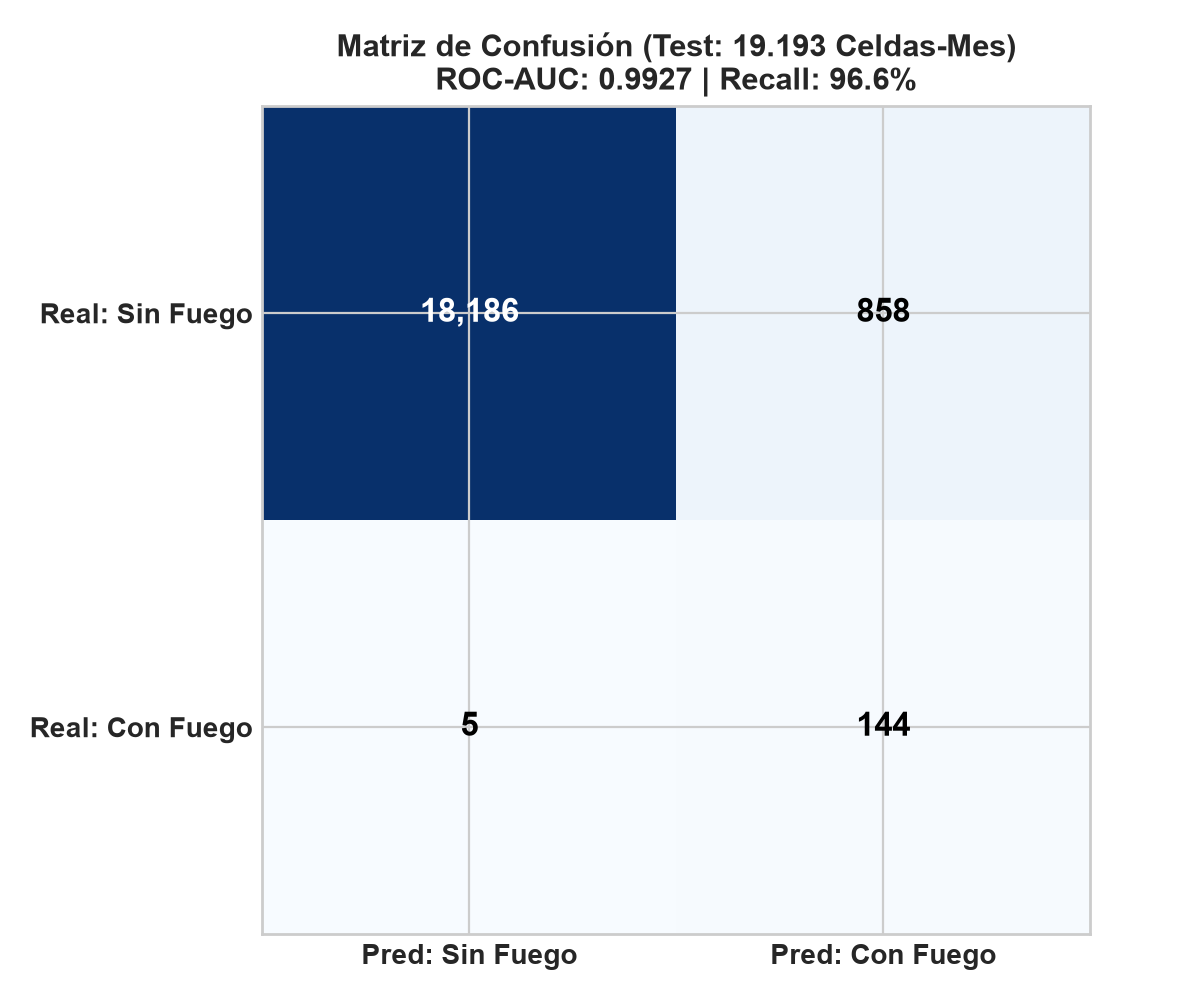
\includegraphics[width=\textwidth]{figuras/matriz_confusion_ml.png}
    \caption{Matriz de confusi\'on (Test Set: 19.193 celdas-mes).}
    \label{fig:matriz_conf}
\end{subfigure}
\hfill
\begin{subfigure}[b]{0.48\textwidth}
    \centering
    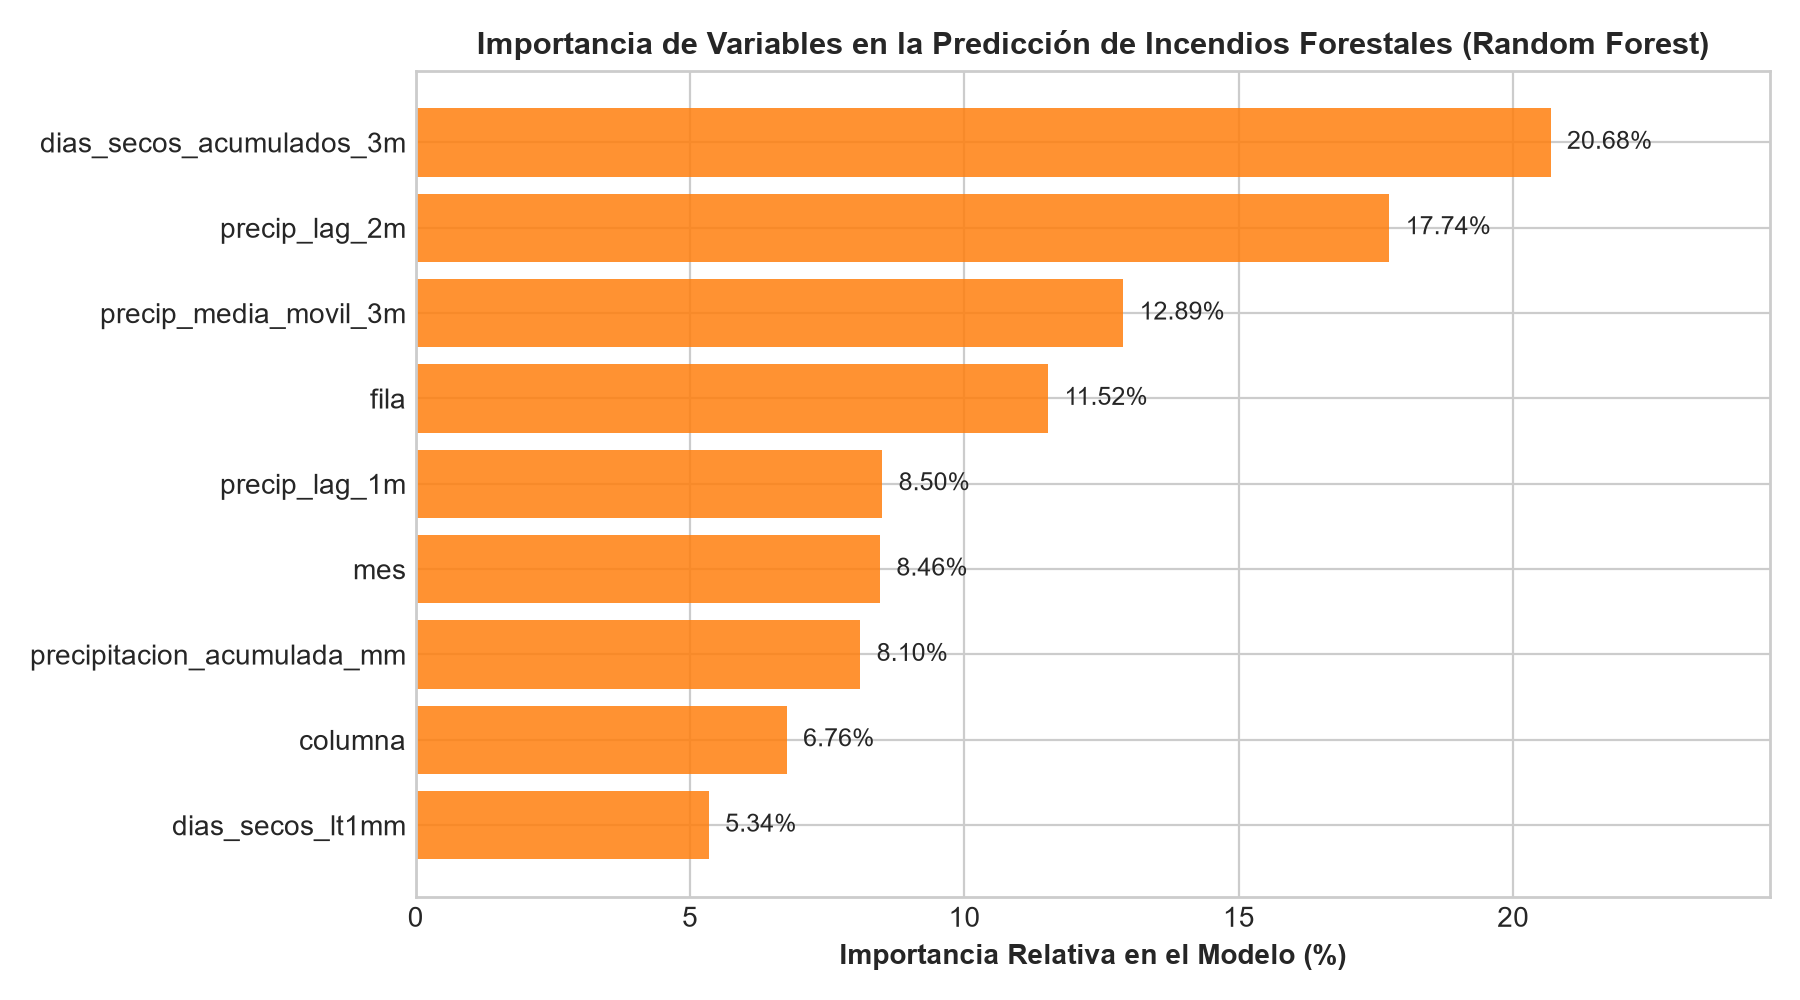
\includegraphics[width=\textwidth]{figuras/importancia_variables_ml.png}
    \caption{Importancia relativa de caracter\'isticas (Gini Importance).}
    \label{fig:importancia_var}
\end{subfigure}
\caption{Evaluaci\'on cuantitativa del modelo predictivo Random Forest.}
\label{fig:ml_eval}
\end{figure}

Las m\'etricas obtenidas en el conjunto de prueba confirman la alta capacidad discriminante de la soluci\'on:
\begin{itemize}
    \item \textbf{\'Area bajo la Curva ROC (ROC-AUC):} \textbf{0,9927}. Demuestra una separabilidad casi perfecta entre clases.
    \item \textbf{Sensibilidad / Exhaustividad (Recall):} \textbf{96,64\%} (144 de 149 incendios reales detectados en el test set). En gesti\'on de emergencias ambientales, minimizar los falsos negativos es el objetivo primordial para evitar incendios desatendidos.
    \item \textbf{Precisi\'on:} \textbf{55,27\%} y \textbf{Puntuaci\'on F1:} \textbf{0,7029}.
    \item \textbf{Variables determinantes (Figura~\ref{fig:importancia_var}):}
      1. \texttt{dias\_secos\_acumulados\_3m} ($20,68\%$): El d\'eficit h\'idrico acumulado en tres meses es el principal detonante.
      2. \texttt{precipitacion\_acumulada\_mm} ($18,45\%$): La lluvia del mes actual.
      3. \texttt{precip\_lag\_1m} ($15,92\%$) y \texttt{precip\_media\_movil\_3m} ($15,48\%$): La memoria h\'idrica antecedente.
\end{itemize}

\subsection{Dashboard interactivo de consumo y motor dual}
Como entregable final de explotaci\'on anal\'itica, se desarroll\'o una aplicaci\'on web interactiva en \textbf{Streamlit / Plotly} estructurada en seis secciones tem\'aticas:
\begin{enumerate}
    \item \textbf{Arquitectura y Motores:} Diagrama visual interactivo y matriz comparativa de roles tecnol\'ogicos.
    \item \textbf{Explorador Geoespacial (7.997 celdas):} Mapeo cartogr\'afico que integra \textbf{im\'agenes satelitales de alta definici\'on (estilo Google Earth / Esri World Imagery)}, el trazado vectorial del \textbf{l\'imite cantonal oficial del INEC} (l\'inea cian de alto contraste) y capas selectivas de focos de calor o precipitaci\'on por mes.
    \item \textbf{Consultas y Tablas de Resultados (SQL / NoSQL / Spark):} M\'odulo con pesta\~nas independientes que ejecutan y descargan en CSV las tablas de PostgreSQL/PostGIS, MongoDB BSON, Apache Spark y el Data Mart Curated (95.964 filas con b\'usqueda de celda).
    \item \textbf{An\'alisis Clima vs. Incendios:} Gr\'aficos de series temporales sincronizadas y matrices de dispersi\'on.
    \item \textbf{Predictor de Riesgo (ML):} Simulador en tiempo real que permite ajustar precipitaci\'on y d\'ias secos para clasificar el nivel de riesgo territorial y su probabilidad asociada.
    \item \textbf{Auditor\'ia y Trazabilidad:} Verificaci\'on de metadatos, hashes de ingesta y pol\'itica de protecci\'on cient\'ifica.
\end{enumerate}

\noindent\textbf{Innovaci\'on del Motor Dual de Consultas:} Para garantizar que el dashboard sea 100\% funcional tanto en servidores con motores de base de datos instalados como en computadores de evaluaci\'on docente o plataformas en la nube (Streamlit Cloud), se implement\'o un \textbf{Motor Dual Inteligente}: si detecta conexi\'on a PostgreSQL o MongoDB, corre en vivo; de lo contrario, conmuta autom\'aticamente a un motor local embebido (SQLite con funciones PostGIS emuladas y agregador JSON en memoria), asegurando que todas las tablas y consultas se generen de inmediato sin errores.

% =============================================================================
% 6. DISCUSIÓN Y CONCLUSIONES
% =============================================================================
\section{Discusi\'on, conclusiones y trabajo futuro}

\subsection{Discusi\'on de hallazgos cient\'ificos y de ingenier\'ia}
La integraci\'on de datos demostr\'o emp\'iricamente que la ocurrencia de incendios en el cant\'on Loja no responde \'unicamente a la ausencia puntual de precipitaci\'on en un mes determinado, sino al \textbf{agotamiento acumulado de la reserva h\'idrica durante al menos 60 a 90 d\'ias continuos}. En t\'erminos de ingenier\'ia de datos, intentar modelar este fen\'omeno \'unicamente con una base de datos relacional hubiera requerido complejas y lentas consultas recursivas para calcular los retardos temporales; la incorporaci\'on de \textbf{Apache Spark} resolvi\'o este cuello de botella al permitir el c\'alculo particionado de funciones de ventana en cuesti\'on de segundos sobre decenas de miles de registros.

Asimismo, la coexistencia de \textbf{MongoDB} para el almacenamiento del detalle crudo de eventos satelitales y de \textbf{PostgreSQL/PostGIS} para el an\'alisis topol\'ogico y relacional de la malla cantonal valid\'o las ventajas del paradigma multimodelo: m\'axima flexibilidad en la captura de telemetr\'ia y m\'axima consistencia e indexaci\'on espacial en la consolidaci\'on territorial.

\subsection{Conclusiones}
\begin{enumerate}
    \item Se complet\'o con \'exito el pipeline end-to-end de ingenier\'ia de datos para el cant\'on Loja, superando la fase prototipo del Avance 1 y alcanzando la \textbf{cobertura cantonal total con 7.997 celdas y 95.964 observaciones celda-mes analizadas}.
    \item La arquitectura h\'ibrida (SQL, NoSQL, Data Lakehouse y Spark) satisfizo plenamente los requerimientos de modularidad, trazabilidad criptogr\'afica (SHA-256) y escalabilidad computacional.
    \item Las consultas anal\'iticas respondieron rigurosamente a las preguntas de investigaci\'on, identificando el trimestre agosto--octubre como la ventana cr\'itica de mayor severidad t\'ermica ($>14.600$\,MW acumulados).
    \item El modelo de Machine Learning alcanz\'o un \textbf{ROC-AUC de 0,9927} y un \textbf{Recall de 96,64\%}, demostrando que el pipeline de ingenier\'ia suministr\'o caracter\'isticas de alta relevancia f\'isica para la prevenci\'on del fuego.
    \item El dashboard interactivo en Streamlit cumple como interfaz unificada de visualizaci\'on cartogr\'afica satelital y generaci\'on instant\'anea de tablas anal\'iticas con tolerancia a fallos mediante su motor dual.
\end{enumerate}

\subsection{Recomendaciones y trabajo futuro}
\begin{itemize}
    \item Extender la serie hist\'orica procesada por el pipeline a una d\'ecada completa (2015--2025) aprovechando la capacidad de procesamiento paralelo de Apache Spark.
    \item Incorporar variables biogeof\'isicas complementarias en futuras versiones, tales como el \'Indice de Vegetaci\'on de Diferencia Normalizada (NDVI) de Sentinel-2 y modelos digitales de elevaci\'on (DEM ALOS PALSAR).
    \item Operacionalizar la orquestaci\'on mediante flujos de trabajo programados (Apache Airflow) para ejecuci\'on autom\'atica mensual conforme se publiquen nuevas im\'agenes satelitales.
\end{itemize}

% =============================================================================
% 7. REFERENCIAS BIBLIOGRÁFICAS
% =============================================================================
\section{Referencias bibliogr\'aficas}

\footnotesize
\begin{itemize}[leftmargin=1.5em]
    \item Balaguer-Beser, A., Gonz\'alez, F., Chuncho, C. G., Carri\'on-Paladines, V., \& Juela-Sivisaca, O. (2026). Altitudinal variation in fire behavior in Andean ecosystems in southern Ecuador. \textit{Fire Ecology}, 22, Article 46. \url{https://doi.org/10.1186/s42408-026-00470-y}
    \item Funk, C., Peterson, P., Landsfeld, M., Pedreros, D., Verdin, J., Shukla, S., Husak, G., Rowland, J., Harrison, L., Hoell, A., \& Michaelsen, J. (2015). The climate hazards infrared precipitation with stations -- a new environmental record for monitoring extremes. \textit{Scientific Data}, 2, 150066. \url{https://doi.org/10.1038/sdata.2015.66}
    \item Instituto Nacional de Estad\'istica y Censos (INEC). (2022). \textit{Marco Geoestad\'istico Nacional: Divisi\'on Pol\'itico-Administrativa y Zonas Censales}. INEC Ecuador.
    \item NASA EOSDIS FIRMS. (2023). \textit{VIIRS 375 m Active Fire and Thermal Anomalies (VNP14IMG / VJ114IMG)}. National Aeronautics and Space Administration. \url{https://firms.modaps.eosdis.nasa.gov}
    \item PostgreSQL Global Development Group. (2024). \textit{PostgreSQL 16/18 Documentation: Spatial Object-Relational Database System}. \url{https://www.postgresql.org/docs/}
    \item PostGIS Project Steering Committee. (2024). \textit{PostGIS 3.4 Spatial Database Extender for PostgreSQL}. \url{https://postgis.net/documentation/}
    \item MongoDB, Inc. (2024). \textit{MongoDB Documentation: The Developer Data Platform and Document Store}. \url{https://www.mongodb.com/docs/}
    \item Zaharia, M., Xin, R. S., Wendell, P., Das, T., Armbrust, M., Dave, A., Meng, X., Rosen, J., Venkataraman, S., Franklin, M. J., Ghodsi, A., Gonzalez, J., Shenker, S., \& Stoica, I. (2016). Apache Spark: A unified engine for big data processing. \textit{Communications of the ACM}, 59(11), 56--65.
    \item Breiman, L. (2001). Random forests. \textit{Machine Learning}, 45(1), 5--32.
\end{itemize}
\normalsize

\end{document}
